\documentclass[12pt]{article}
%article: Documentos cortos
%book: Hacer libros(Capítulos, apéndices)
%report: Documentos MUY cortos
%memoir: Todo en 1

%Más fuentes en 
%https://community.rstudio.com/t/cant-creat-pdf-cant-find-tinytex-or-miktex-files/34960
%https://tug.org/FontCatalogue/mathfonts.html

%12pt: Tamaño de letra de 12 puntos
%twocolumns: Doble columna
\usepackage{ 
graphicx,       %Para meter figuritas
enumitem,       %Para hacer listas chidas (Paquete esencial en la vida)
amsfonts,       %Las letras de pizarra
amsmath,        %Fracciones, integrales y otras cosas
amsthm,         %Teoremas
amssymb,        %Más símbolos
mathtools,      %MÁS SÍMBOLOS
mathrsfs,       %Letras cursivas matemáticas
bm,             %Letras matemáticas negritas
bbm,            %Esta da la indicadora con \mathbbm 1
actuarialsymbol,%Símbolos actuariales
physics         %Símbolos físicos
}
\usepackage[ruled,vlined,spanish,onelanguage]{algorithm2e} %Algoritmos
\usepackage[utf8]{inputenc}
% Para que el documento pueda poner acentos y demás caracteres.
\title{La tarea que pidió Imanol} %Aquí va el título
\author{Pues yo, quién más}  %El autor
\date{Hoy} %La fecha

\setlength\parindent{0pt}
%Quitar sangría
\begin{document}
\maketitle %Aquí pedimos que se ponga el título, autor y fecha
añ 

\begin{abstract}
	En este documento vamos a aprender a usar \LaTeX (\TeX).
\end{abstract}


A en unicode (U+0041). \textbf{Así ponemos las letras negritas}. \emph{Así las itálicas} o \textit{así}. \underline{Así subrayamos cosas}. \textbf{\underline{llll}}.\\
\section{Lista del súper}
\begin{itemize}
\item[$\square$] Zanahorias, 
\item[c)] Aguacate,
\item Manzanas,
\item Naranjas,
\item $\frac{1}{2}$kg de fresas, %Así se ponen las fracciones chiquitas dentro del texto
\item $\dfrac{1}{4}$kg queso parmesano.%Así se ponen las fracciones grandes dentro del texto
\end{itemize}

\section{Pasos para superar el alcoholismo}
\begin{enumerate}
\item Aceptar que tienes un problema.
\item Ir a tomar café con @ImanolBuscaTag.
\end{enumerate}

\subsection{Lista del súper}
\begin{itemize}[label=$\square$]
\item Zanahorias, 
\item Aguacate,
\item Manzanas,
\item Naranjas,
\item $\frac{1}{2}$kg de fresas, %Así se ponen las fracciones chiquitas dentro del texto
\item $\dfrac{1}{4}$kg queso parmesano.%Así se ponen las fracciones grandes dentro del texto
\end{itemize}

%\part{}  Éste no sirve para archivos tipo article
%\chapter{} Éste tampoco
%\section{}
%\subsection{}
%\subsubsection{}
%\paragraph{}    No lo vamos a ocupar
%\subparagraph{}     Tampoco


A + ` = À

?`% Así se pone el caracter ¿

\'a %Poner acento
\\ %Salto de línea
Sea $f:[a,b]\to\mathbb R$ una función continua y $F:[a,b]\to\mathbb R$ una función tal que $F'(x)=f(x),$ para toda $x\in [a,b]$, entonces
\[\int_a^b f(x) \, \text{d}x = F(b)-F(a)\ax[n|]{x} .\] %Fórmulas en grande
\[\actsymb[n]{A}{x} \]
\[\dv[n]{f}{x}  \]
\[3.14^2\pdv[2]{u}{x} =  \pdv[2]{u}{t}\]



efeaxwqx

\begin{algorithm}[h]
\KwData{$n$ un número natural.}
\KwResult{ El \begin{math}n\end{math}-ésimo término de la sucesión de Fibonacci.}
$aux=n$\,
\If{aux = 0,1}{
regresa 1
}{
Fibonacci($aux-1$)+Fibonacci($aux-2$)
}
\caption{Fibonacci}
\end{algorithm}


\begin{algorithm}[H]
 \KwData{Una matriz $C$ de costos.}
 \KwResult{$\overline U$ conjunto inicial de asignaciones,\\ $\varphi$ un inicial vector de asignación de personas,\\ $f$ un vector inicial de asignación de tareas,\\$(u,v)$ una solución dual factible.}
  \For{$i \in\{1,...,n\}$}{
   $u_i := \min\{c_{i,j}:j\in\{1,...,n\}\}$\;
   }
  \For{$j \in\{1,...,n\}$}{
   $v_j := \min\{c_{i,j}-u_i : i\in\{1,...,n\}\}$
   }
  \For{$i \in\{1,...,n\}$}{
   \For{$j \in\{1,...,n\}$}{
    \If{$f(j) = 0$, $c_{i,j}-u_i-v_j=0$ y $i\notin\overline U$ }{
    $f(j) = i$\;
    $\varphi(i) = j$\;
    $\overline U = \overline U \cup \{i\}$
    }
   }
  }
 \caption{Preprocesamiento}
\end{algorithm}

\begin{figure}[htp]
\centering
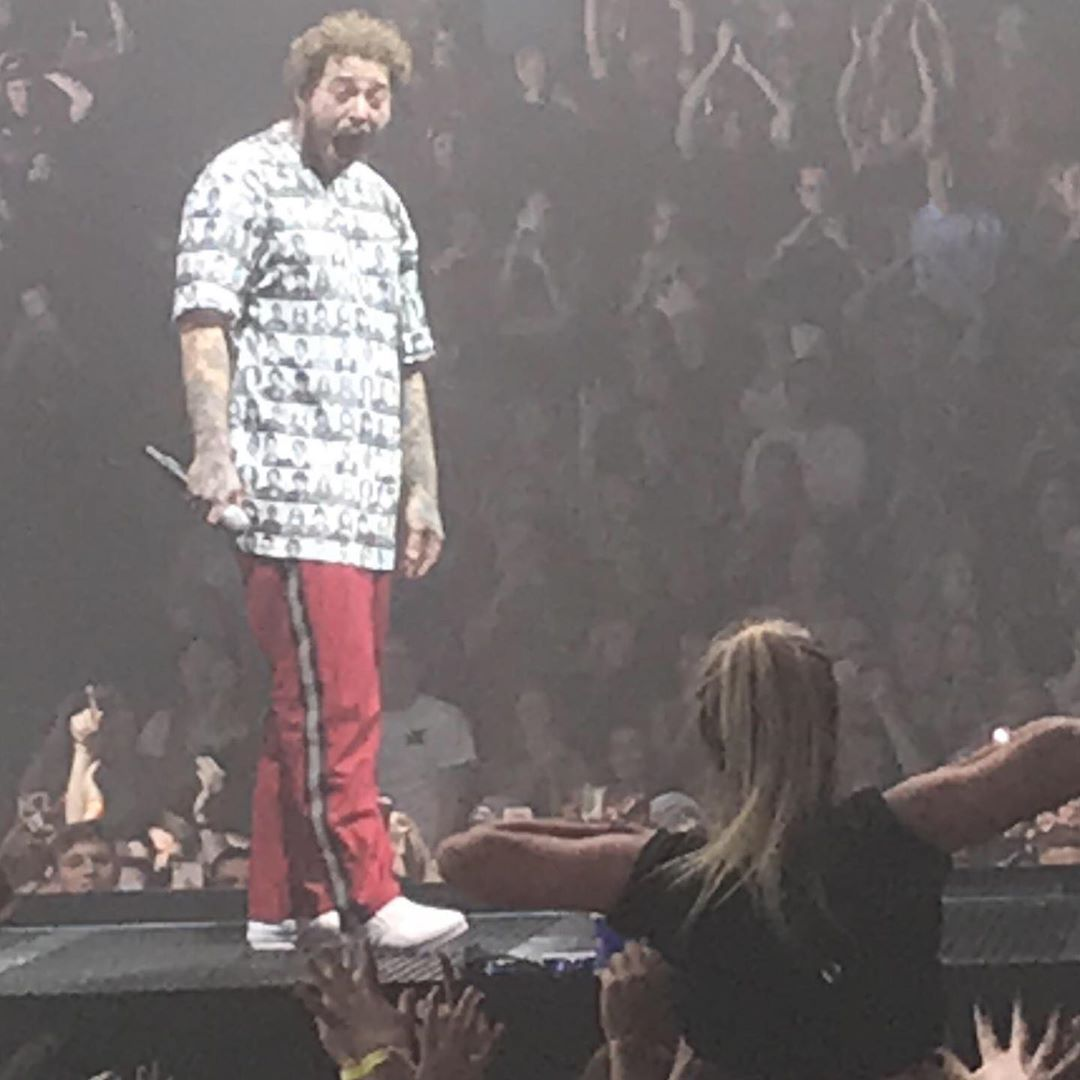
\includegraphics[scale = 0.1]{lol}
\caption{looool}
\end{figure}


5tef
erger
\end{document}